%%%--------------------------------%%%
%%% UC7
%%%--------------------------------%%%

\newpage
% UC7 ====================================================
\subsubsection{Use Case Specification: \ac{UC}7 Risk Monitoring}
\label{sec:domainBbh}

\paragraph*{Description}\mbox{}\\
This \ac{UC} deals with the monitoring of risks. It enables reminding the project team and its members to take care of the defined risks.

\paragraph*{Basic Flow} \mbox{}\\
\noindent
The risks' response defines if the described reaction has to be done just once or on a regular basis. 

\noindent
One-time:
\begin{itemize}
	\vspace{-3mm}
	\setlength\itemsep{-1em}	
	\item When adding a response to a risk which is only processed one time the user can set a fixed date until when the response should be taken care of.
	\item Before the deadline the person in charge is notified. "Have you already handled <the response> (Yes | No)".
\end{itemize}

\noindent
Regular basis:
\begin{itemize}
	\vspace{-3mm}
	\setlength\itemsep{-1em}
	
	\item When adding a response to a risk which is processed on a regular basis the user can set an interval in which the response should be repeated.
	\item The person in charge is notified according to this interval. "Have you already done <the response> (Yes | No)".
\end{itemize}

\begin{figure}[H]
	\centering
	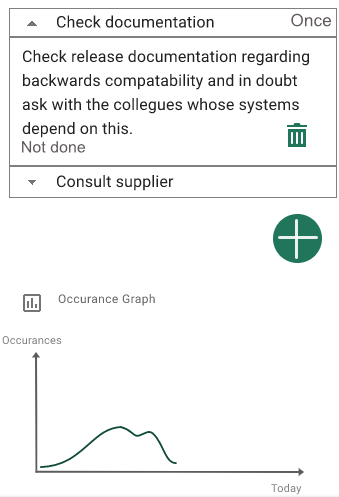
\includegraphics[width=0.3\textwidth]{Assets/UC_Screenshots/UC7S.png}
	\caption{Use Case 7: Mock Prototype}
	\label{fig:useCase7Detail}
\end{figure}

\paragraph*{Special Requirements and Preconditions}\mbox{}\\
The preconditions for this use case are:
\begin{enumerate}
	\vspace{-3mm}
	\setlength\itemsep{-1em}
	
	\item A project exists.
	\item The user is member of the project.
	\item The user is the person in charge of a risk.
\end{enumerate}

\paragraph*{Postconditions and Persistence}\mbox{}\\
The postconditions for this use case are:
\begin{enumerate}
	\vspace{-3mm}
	\setlength\itemsep{-1em}
	
	\item Best case: The risk's response was done and the user in charge is rewarded.
	\item Undesired case: The risk's response was not done by the deadline and the user in charge is 'punished'.
\end{enumerate}

\subparagraph{Activity Diagram}\mbox{}\\
\begin{figure}[H]
	\centering
	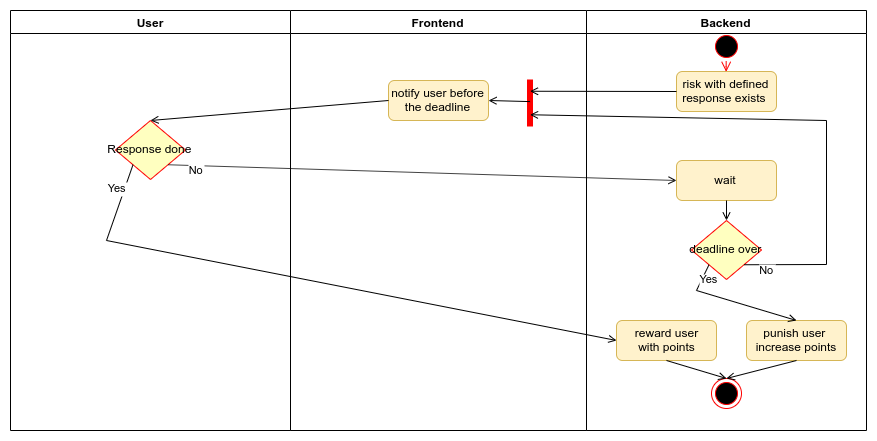
\includegraphics[width=1.0\textwidth]{Content/Domain/UC7RiskMonitoring.png}
	\caption{Activity Diagram \ac{UC}7 Risk Monitoring}
	\label{fig:label77}
\end{figure}